\documentclass[a4paper]{report}
\usepackage{fullpage}
\usepackage{amssymb}
\usepackage{amsmath}
\usepackage{graphicx}
\usepackage{tikz}
\usepackage{tocbibind}
\usepackage{subcaption}
%\usepackage{subfig}
\usepackage{caption}
\usepackage{listings}
\usepackage{lipsum}
\usepackage{mdframed}
\usepackage{url}
\usepackage{cite}
\usepackage{dirtytalk}

\title{Business Management Processes: Verifying their Compliance with Security and Business Rules}
\author{Joanna Diep}
\begin{document}
\bibliographystyle{unsrt}
\begin{titlepage}
\newcommand{\HRule}{\rule{\linewidth}{0.5mm}} % Defines a new command for the horizontal lines, change thickness here

\center % Center everything on the page

\textsc{\LARGE Imperial College London}\\[1.5cm] % Name of your university/college
\textsc{\Large Individual Project Report}\\[0.5cm] % Major heading such as course name
\textsc{\large Department of Computing}\\[0.5cm] % Minor heading such as course title

\HRule \\[0.4cm]
{ \huge \bfseries Business Management Processes: Verifying their Compliance with Security and Business Rules}\\[0.4cm] % Title of your document
\HRule \\[1.5cm]
 
\begin{minipage}{0.4\textwidth}
\begin{flushleft} \large
\emph{Author:}\\
Joanna \textsc{Diep} 
\end{flushleft}
\end{minipage}
~
\begin{minipage}{0.4\textwidth}
\begin{flushright} \large
\emph{Supervisor:} \\
Professor. Michael \textsc{Huth} \\ 
\emph{Second Marker:} \\
Dr. Anandha \textsc{Gopalan} 
\end{flushright}
\end{minipage}\\[4cm]


\includegraphics[scale=0.15]{Imperial_College_London_crest.png}\\[1cm]

{\large \today}\\[3cm] % Date, change the \today to a set date if you want to be precise
 
\vfill % Fill the rest of the page with whitespace
\end{titlepage}

\begin{abstract}
TODO\\
\end{abstract}

\renewcommand{\abstractname}{Acknowledgements}
\begin{abstract}
I would like to whole heartedly thank my supervisor Professor. Michael Huth for his continuous and invaluable advice, feedback and support throughout the course of this project. As well as giving time for meetings to discuss ideas. \\
I would like to thank Dr. Anandha Gopalan, the second marker for their feedback and suggestions to greatly improve my report. \\
Finally, I would like to thank my family and friends for their love, support and who have had to put up with me throughout this project and throughout my time at Imperial College.  
\end{abstract}

\tableofcontents

\chapter{Introduction}

\chapter{Background}
\section{Workflows}
\setlength{\parindent}{4em}
Business management processes can be represented as a workflow of tasks, where each of these tasks produce a certain output for the next task to be realised. These tasks are assigned in the workflow as a sequence, where in order to perform the next task, the current task must be completed. However, in order to start a task, it must meet all the constraints within workflow. However, in a large business, making sure that all the constraints are met in a workflow can become a large problem as the more tasks are added to a workflow.   Workflows are modeled as directed acyclic graphs\cite{AcyclicDigraph}, where there are no directed cycles. The vertices are tasks in the workflow and the directed edges connecting to each task vertex is the execution order. \par
\begin{figure}
\centering
\begin{subfigure}[b]{\textwidth}
\centering
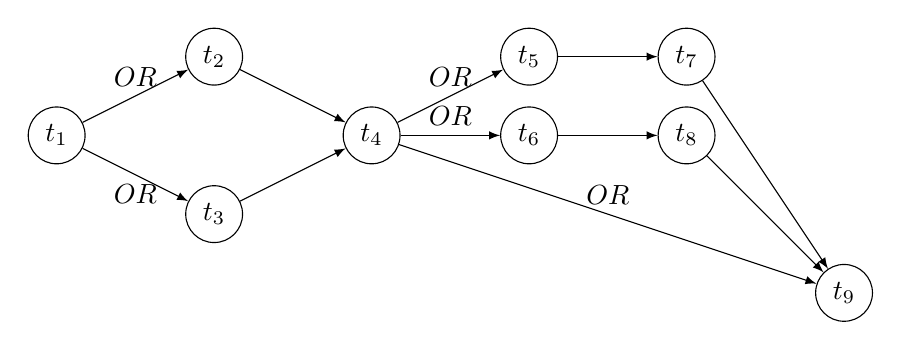
\begin{tikzpicture}
\tikzset{vertex/.style = {shape=circle,draw,minimum size=1.5em}}
\tikzset{edge/.style = {->,> = latex}} 
%\draw (0,0) circle [radius=0.5];
\node[vertex] (a) at  (0,0) {$t_{1}$};
\node[vertex] (b) at  (2,1) {$t_{2}$};
\node[vertex] (c) at (2,-1) {$t_{3}$};
\node[vertex] (d) at (4,0) {$t_{4}$};
\node[vertex] (e) at (6,1) {$t_{5}$};
\node[vertex] (f) at (6,0) {$t_{6}$};
\node[vertex] (g) at (8,1) {$t_{7}$};
\node[vertex] (h) at (8,0) {$t_{8}$};
\node[vertex] (i) at (10,-2) {$t_{9}$};
%\draw[edge] (a) to (b);
%\draw[edge] (a) to (c);
\draw[edge] (b) to (d);
\draw[edge] (c) to (d);
%\draw[edge] (d) to (e);
%\draw[edge] (d) to (f);
%\draw[edge] (d) to (i);
\draw[edge] (e) to (g);
\draw[edge] (f) to (h);
\draw[edge] (g) to (i);
\draw[edge] (h) to (i);
\path[-latex]
(a) edge node[above] {$OR$} (b)
(a) edge node[below] {$OR$} (c)
%(b) edge node[below] {} (d)
%(c) edge node[below] {} (d)
(d) edge node[above] {$OR$} (e)
(d) edge node[above] {$OR$} (f)
(d) edge node[above] {$OR$} (i);
%(e) edge node[below] {} (g)
%(f) edge node[below] {} (h)
%(g) edge node[below] {} (i)
%(h) edge node[below] {} (i);
\end{tikzpicture}
\caption{Ordered business workflow with nine tasks}
\label{fig:Business workflow with nine tasks}
\end{subfigure} \\
\begin{subfigure}[b]{\textwidth}
\centering
\begin{tabular}{ |l|l| }
\hline
Task Number & Task \\ \hline
$t_1$ & Receive order from customer \\ \hline
$t_2$ & Give total of large sale \\ \hline
$t_3$ & Give total of small sale \\ \hline
$t_4$ & Approve and authorise checkout \\ \hline
$t_5$ & Give 10\% discount \\ \hline
$t_6$ & Give 20\% discount \\ \hline
$t_7$ & Give new total of sale \\ \hline
$t_8$ & Give new total of sale \\ \hline
$t_9$ & Approve and return new total \\ 
\hline
\end{tabular}
\caption{Table of tasks}
\label{fig:Table of tasks}
\end{subfigure}
\caption{Business management process workflow}
\label{fig:Business management process workflow}
\end{figure}
An example of a business workflow is given in Figure~\ref{fig:Business workflow with nine tasks} with nine tasks that need to be allocated:
\begin{itemize}
\item A user in the business receives the order from a customer.
\item They then pass it onto another user depending on the two possible sizes of the order and are given different prices accordingly. 
\item Someone then needs to approve and authorise the price for checkout.
\item Then a discount may be provided depending on the current total cost of the order.
\item Finally, the sale is approved and the new total is returned back to the customer.
\end{itemize}

However, the order of of execution in Figure~\ref{fig:Business workflow with nine tasks} is affected by how to graph is forked. These forks are represented as constraints or rules within a business which may prevent tasks being executed such as a government restriction on business logic. The fork at $t_{1}$ is an OR-fork showing that either $t_{2}$ or $t_{3}$ can be executed. Depending on whether $t_{2}$ or $t_{3}$ can be executed, determines whether $t_{4}$ can then be executed afterwards and affects the whole execution of the workflow.  \\

\section{Tasks}
In business management processes, users have to be allocated tasks for an execution to occur. These tasks are represented as vertices in the graph as $t_{n}$. The tasks in the example workflow given in Figure~\ref{fig:Business workflow with nine tasks} are listed in Table~\ref{fig:Table of tasks}.\\
If users cannot be allocated to these tasks, then there is no way in which the task can be executed. Therefore it is not executed and the workflow becomes unsatisfiable.\\

\section{Users}
A user belongs to the set of users who can be allocated to tasks in order to execute them. However, there are possible allocation constraints which refrain particular users from executing these tasks. In the example given below, Alice, Bob and Carol are users specified in the domain of the workflow, but David is not.\\
\begin{center}
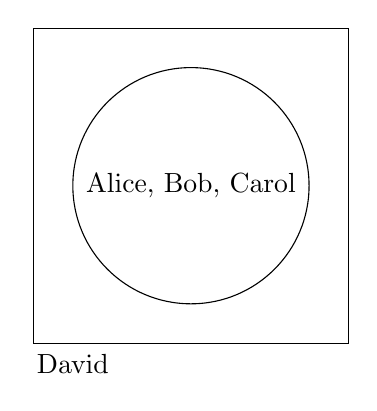
\begin{tikzpicture}
\draw (0,0) -- (4,0) -- (4,4) -- (0,4) -- cycle node[right=0.5cm, below=0.5] {David};
\draw (2,2) circle(1.5cm) node {Alice, Bob, Carol};
\end{tikzpicture}
\end{center}

\section{Business and Security Rules}
Business and security rules are used to prevent fraud and follow business compliance rules. For example, in some cases, different users are needed to execute a certain set of tasks to perhaps prevent fraud or erroneous activities in a workflow. In Figure~\ref{fig:Business management process workflow} some constraints about which users in the business can execute these tasks are added below:
\begin{itemize}
\item Whomever is allocated task $t_{1}$ to receive the order from customers and pass them onto the relevant user, but cannot be allocated and execute $t_{2}$ and $t_{3}$, but can be allocated other tasks within the workflow besides $t_{2}$ and $t_{3}$.
\item Whomever is allocated task $t_{2}$ to give a total of a large sale cannot be the same user that is allocated $t_{3}$ who gives a total of a small sale. Therefore whomever is allocated $t_{3}$ cannot be allocated to $t_{2}$.
\end{itemize}
With the additional constraints to the workflow it may be satisfiable given that there are enough users. But there may be other constraints that can make this workflow unsatisfiable. For example, if there are not enough users to be allocated to ensure that some of the tasks do not have the same user. So a valid workflow is a satisfied workflow if there can be users allocated tasks in the workflow that do not break the constraints within the given model.\\

\section{Satisfiability Modulo Theories (SMT)}
Satisfiability Modulo Theories (SMT)\cite{smt_appetizer} check the satisfiability of logical formulas over given theories. It helps to determine whether there is a solution in a formula which expresses a constraint. It is one of the fundamental problems in the area of computer science to check boolean satisfiability over logical domains and the completeness and incompleteness of logical theories and complexity theory. \\
SMT is similar to Boolean or Propositional Satisfiability Problem (SAT)\cite{sat} , where the problem is to determine if there exists a determination that satisfies the boolean formula. But SAT ranges only over binary predicates which are predicated that only take in two arguments in their formula. Whereas SMT covers non-binary predicates with types and sorts. This project will focus on SMT rather than SAT as we can use non-binary predicates provided by SMT to define and solve some of these constraints. \\

\section{Z3}
Z3\cite{smt} is a SMT solver developed by Microsoft Research. It is used to integrate several decision procedures and verify the satisfiability of logical formulas over given theories. The theories our case, is the workflow model. There are many features of Z3 which will come in useful including:
\begin{itemize}
\item Uninterpreted functions - where a theory has an empty set of sentences. An example of this can be an axiom, where the satisfiability of the axiom depends on whether the uninterpreted function can be evaluated to true.
\item Linear arithmetic
\item Bitvectors, arrays, datatypes
\item Quantifiers
\item Satisfiability core
\item Returns a model
\end{itemize}
There were many other SMT solvers considered but did not include certain built in theories and features such as:
\begin{itemize}
\item Yices\cite{yices} - it has almost all features of Z3 but doesn’t have quantifiers, which is needed to define general rules to satisfy a formula in the domain. 
\item CVC4\cite{cvc4} - Similar features of Z3 including quantifiers not included in Yices. But typically with CVC4, it is not very scalable. It is intended to run with small finite models, but realistically, business processes can be huge within large organisations.
\item MathSAT 5\cite{mathsat5}- It is lacking a lot of features in Z3, especially the quantifiers.
\end{itemize}

\subsection{Basics}
A simple example is illustrated in Figure~\ref{fig:Simple predicate logic} shows how some simple first order predicate logic in Figure~\ref{fig:Simple predicate logic using logic symbols} can be expressed in Z3 SMT solver in  Figure~\ref{fig:Simple predicate logic in Z3}.
\begin{itemize}
\item To define constants in Z3, in this case $x$ and $y$, we can declare them as constants using the keyword \texttt{(declare-const x Int)} where $x$ is the name of the constant and the type of $x$ is an Integer.
\item Z3 uses assertions to add constraints to the solver as a keyword assert. 
\item \texttt{(check-sat)} (line 5) is a call to Z3 to check if the theory is satisfiable. It returns sat is the theory is satisfiable and unsat if the theory is unsatisfiable.
\item \texttt{(get-model)} (line 6) is a call to Z3 to return an interpretation of the theory which makes all the formulas defined in the Z3 stack true. If the theory returns false, no model able to be retrieved.  
\end{itemize}
In the example below, $x > 10$ is given as an assertion \texttt{(assert(> x 10))} and $y \times 10 \geq x$ is given the assertion \texttt{(assert (>= (* y 10) x))}. When this is run in Z3, a result is returned. \texttt{(check-sat)} returns as sat which means that this theory is satisfiable.\\ 
What we can see also, is that Z3 gives back an appropriate model as a result that satisfies these constraints with $x = 11$ and $y = 2$. This is true as if we put $x = 11$ and $y = 2$ back into the constraints, $11 > 10$ and $20 \geq 11$.
\begin{figure}[!htb]
\centering
\begin{subfigure}[b]{\textwidth}
\centering
$x > 10$ \\
$y \times 10 \geq x$
\caption{Simple predicate logic using logic symbols}
\label{fig:Simple predicate logic using logic symbols}
\end{subfigure}
\begin{subfigure}[b]{\textwidth}
\lstset{numbers=left, showspaces=false,
    showstringspaces=false, tabsize=2, breaklines=true,
    xleftmargin=5.0ex,
}
\centering
%\begin{figure}[!htb]
%  \lstset{numbers=left, showspaces=false,
%    showstringspaces=false, tabsize=2, breaklines=true,
%    xleftmargin=5.0ex,
    %numberstyle=\scriptsize,numbersep=0pt
%}
%$x > 10$ \\
%$y \times 10 \geq x$
\begin{lstlisting}[frame=single]
(declare-const x Int)
(declare-const y Int)
(assert (> x 10))
(assert (>= (* y 10) x))
(check-sat)
(get-model)
\end{lstlisting}
\caption{Simple predicate logic in Z3}
\label{fig:Simple predicate logic in Z3}
\end{subfigure}\\
%\end{center}
%Z3 returns a model:
%\begin{center}
\begin{subfigure}[b]{0.3\textwidth}
\begin{lstlisting}
sat
(model 
  (define-fun y () Int
    2)
  (define-fun x () Int
    11)
)
\end{lstlisting}
\caption{Z3 Result}
\label{fig:Z3 Result}
\end{subfigure}
\caption{Simple predicate logic}
\label{fig:Simple predicate logic}
\end{figure}

\subsection{Functions}
Z3 also has uninterpreted functions where unlike most programming languages where functions have side effects, may never return a value or raise or throw exceptions, Z3 functions have no side effects since they are in classical first order logic and are total.
Everything in Z3 is a function, including constants as they don’t take in arguments.
\begin{itemize}
\item \texttt{(declare-fun f (Int) Int)} - We declare a function $f$ which takes in and integer as its parameter and returns an integer
\end{itemize}
In Figure~\ref{fig:Predicate Logic with Functions}, a function \texttt{f} has been declared which takes an integer as input, and returns an integer. Since this is an uninterpreted function, Z3 does not know what this function does. But we can add some constraints, so when we apply the function to the integer, it ensures that the interpretation is consistent within the theory and constraints. \\
In Figure~\ref{fig:Z3 with functions}, there are two assertions \texttt{(assert (= (f x) x))} which represents $f(x) = x$ and \texttt{(assert (> (f y) (f x))} as $f(f) > f(x)$. The result that Z3 returns in Figure~ref{Z3 Result with functions} has still kept the values of \texttt{x} and \texttt{y} as it is the same as Figure~\ref{fig:Simple predicate logic}. But for function $f$, it takes in an integer as we have specified in our function declaration as \texttt{(x!1 Int)} which means that the first variable has a type Int (integer). It returns an integer which is consistent and the type integer is interpreted. \\
Looking at the model returned in Figure~\ref{fig:Z3 Function Result}, we can see that \texttt{x} and texttt{y} are both interpreted as a function as well as texttt{f}. It interprets \texttt{f} to take in an integer, the \texttt{ite} stands for “if-then-else”. So we can read the definition of \texttt{f} as “if x!1 is equal to 20, then return 20, else if x!1 is equal to 2, then return 2 else, return 21. Else, return 20”. So for the case that \texttt{x} is put into the function \texttt{f}, then $x!1 = 20$, then the value of the function is 20, else if \texttt{y} is put into the function, then $x!1 = 2$, then the value of the function is 21. If any other input is put in, then it will return 20. \\
Z3 also includes built in arithmetic functions such as $=, -, +, \times, div, mod, \geq, \leq, >, <, not$ that support integer and real constants. \\

\begin{figure}[!htb]
\centering
\begin{subfigure}[b]{\textwidth}
\centering
$x > 10$ \\
$y \times 10 \geq x$ \\
$f(x) = x$ \\
$f(y) > f(x)$
\caption{Predicate logic with functions}
\label{fig:Predicate logic with functions}
\end{subfigure}
\begin{subfigure}[b]{\textwidth}
\lstset{numbers=left, showspaces=false,
    showstringspaces=false, tabsize=2, breaklines=true,
    xleftmargin=5.0ex,
}
\centering
\begin{lstlisting}[frame=single]
(declare-const x Int)
(declare-const y Int)
(assert (> x 10))
(assert (>= (* y 10) x))
(declare-fun f (Int) Int)
(assert (= (f x) x))
(assert (> (f y) (f x)))
(check-sat)
(get-model)
\end{lstlisting}
\caption{Z3 with functions}
\label{fig:Z3 with functions}
\end{subfigure}\\
\begin{subfigure}[b]{\textwidth}
\begin{lstlisting}[frame=single]
sat
(model 
  (define-fun y () Int
    2)
  (define-fun x () Int
    20)
  (define-fun f ((x!1 Int)) Int
    (ite (= x!1 20) 20
    (ite (= x!1 2) 21
      20)))
)
\end{lstlisting}
\caption{Z3 Result with functions}
\label{fig:Z3 Function Result}
\end{subfigure}
\caption{Predicate Logic with Functions}
\label{fig:Predicate Logic with Functions}
\end{figure} 

\subsection{Stack}
Z3 has a stack implementation, where constraints and formulas can be pushed onto and popped off the stack using the commands \texttt{(push)} and \texttt{(pop)} which pushes and pops constraints off the stack respectively. These commands can be used to check the satisfiability of some rules or definitions. When the solver stack is pushed, the state of the solver is saved. When the stack is popped, any rules and assertions declared between that pop and the corresponding push on the stack is removed from the stack, and the interpretation is reverted back to its previous state before the push.\\
In Figure~\ref{fig:Predicate Logic with stack}, the theory is satisfied before the push. However, when the stack is pushed and an assertion is added which violates the constraints already in the current frame which is $x < 2$, but $x > 2$ has been pushed onto the stack frame previously, the model becomes unsatisfied. Since the constraint $x < 2$ was between a push-pop frame, it can be popped off the stack and the model is returned back to its previous state on the stack.\\
\begin{figure}[!htb]
\centering
\begin{subfigure}[b]{\textwidth}
\lstset{numbers=left, showspaces=false,
    showstringspaces=false, tabsize=2, breaklines=true,
    xleftmargin=5.0ex,
}
\centering
\begin{lstlisting}[frame=single]
(declare-const x Int)
(declare-const y Int)
(declare-fun f (Int) Int)
(assert (> x 2))
(assert (< y 2))
(assert (= (f x) (f y)))
(check-sat)
(get-model)
(push)
(assert (< x 2))
(check-sat)
(pop)
(check-sat)
(get-model)
\end{lstlisting}
\caption{Z3 with stack}
\label{fig:Z3 with stack}
\end{subfigure}\\
\begin{subfigure}[b]{\textwidth}
\begin{lstlisting}[frame=single]
sat
(model 
  (define-fun y () Int
    0)
  (define-fun x () Int
    3)
  (define-fun f ((x!1 Int)) Int
    (ite (= x!1 3) 1
    (ite (= x!1 0) 1
      1)))
)
unsat
sat
(model 
  (define-fun y () Int
    0)
  (define-fun x () Int
    3)
  (define-fun f ((x!1 Int)) Int
    (ite (= x!1 3) 1
    (ite (= x!1 0) 1
      1)))
)
\end{lstlisting}
\caption{Z3 Result with stack}
\label{fig:Z3 Function stack}
\end{subfigure}
\caption{Predicate Logic with stack}
\label{fig:Predicate Logic with stack}
\end{figure} 

\subsection{Sorts}
When a constant is defined, they are declared as a type which is a sort in Z3. For example, integers, reals and booleans are declared, they are a pre-defined sort in Z3. 
\begin{itemize}
\item \texttt{(define-sort t1 Task)} - the command defines a new symbol with the type Task.
\end{itemize}

\subsection{Quantifiers}
One of the reasons why we chose Z3 as the back end constraint solver was because it is able to have quantifiable logic such as the universal quantifier which is interpreted as \say{for all} $\forall$. The universal quantifier asserts that all predicates within the scope of the quantifier must be true of every value of the predicate. In Z3, they are represented as:
\begin{itemize}
\item \texttt{(assert (forall ((x Int)) (x > 0)))} which in first order predicate logic is $\forall x: (x > 0)$. So for all integers, they must be greater than zero.
\end{itemize}

\subsection{Satisfiability and Validity}
\subsubsection{Validity}
A formula $f$ is valid if $f$ always evaluates to true for any assignment to an appropriate value. 
\subsubsection{Satisfiability}
A formula f is satisfiable if there is some assignment to an appropriate value to the function where f evaluates to true.\\
As we mentioned previously, Z3 SMT Solver gives back the satisfiability of the interpretation. It has three states when the (check-sat) command is called:
\begin{itemize}
\item \texttt{sat} - satisfied model, a model can be returned. We give an example of a satisfied formula in Figure~\ref{fig:Z3 with satisfied core}.
\item \texttt{unsat} - unsatisfied model - a model cannot be returned. We give an example of an unsatisfied formula in Figure~\ref{fig:Z3 with unsatisfied core}.
\item \texttt{unknown} - when Z3 does not know whether a formula is satisfiable or not. We give an example of an unknown result in Figure~\ref{fig:Z3 with unknown}.
\end{itemize}
What is good about whether a formula is satisfiable is that it is about finding a solution under a set of constraints. 
\begin{figure}[!htb]
\centering
\begin{subfigure}[b]{\textwidth}
\lstset{numbers=left, showspaces=false,
    showstringspaces=false, tabsize=2, breaklines=true,
    xleftmargin=5.0ex,
}
\centering
\begin{lstlisting}[frame=single]
(declare-const x Int)
(assert (> x 10))
(assert (< x 100))
(check-sat)
(get-model)
\end{lstlisting}
\caption{Z3 with satisfied core}
\label{fig:Z3 with satisfied core}
\end{subfigure}\\
\begin{subfigure}[b]{\textwidth}
\lstset{numbers=left, showspaces=false,
    showstringspaces=false, tabsize=2, breaklines=true,
    xleftmargin=5.0ex,
}
\begin{lstlisting}[frame=single]
(declare-const a Int)
(assert (> a 10))
(assert (< a 10))
(check-sat)
(get-model)
\end{lstlisting}
\caption{Z3 with unsatisfied core}
\label{fig:Z3 with unsatisfied core}
\end{subfigure}
\begin{subfigure}[b]{\textwidth}
\lstset{numbers=left, showspaces=false,
    showstringspaces=false, tabsize=2, breaklines=true,
    xleftmargin=5.0ex,
}
\begin{lstlisting}[frame=single]
(declare-const a Int)
(assert (> a 10))
(assert (< a 10))
(check-sat)
(get-model)
\end{lstlisting}
\caption{Z3 with unknown}
\label{fig:Z3 with unknown}
\end{subfigure}
\caption{Predicate Logic with stack}
\label{fig:Predicate Logic with stack}
\end{figure} 

\chapter{Theory of Business Rules}
\section{Business Management Workflows}
There are many rules and restrictions within business management workflows in order to prevent fraud, and a matter of authorisation and following regulation. Each rule is different, and therefore will have different axioms that follow. We will talk about the rules that have been implemented in the application.\\

\section{Tasks and Users}
Firstly, tasks and users need to be defined in the application in order to define the basic workflow domain. These are defined in Z3 as sorts where they define the types task and user respectively:
\begin{itemize}
\item \texttt{(declare-sort Task)}
\item \texttt{(declare-sort User)}
\end{itemize}
Then each task and user in the domain are able to be defined after the sort has been defined: \\
\lstset{numbers=left, showspaces=false,
    showstringspaces=false, tabsize=2, breaklines=true,
    xleftmargin=5.0ex,
}
\begin{lstlisting}[frame=single]
(declare-sort Task)
(declare-sort User)
(declare-const alice User)
(declare-const bob User)
(declare-const price_large_order Task)
(declare-const price_small_order Task)
\end{lstlisting}
We have now declared a user called \say{alice} and another user \say{bob} in the user domain, as well as defining two tasks in the task domain \say{receive\_large\_order} and \say{recieve\_small\_order}. 

\subsection{User Allocation}
The most basic constraint in a workflow is that the tasks can only be executed if they have been allocated a user. Obviously, if there was not a user in the domain able to be allocated to a task, no one is able to execute and complete the task for the workflow to progress.\\
In Z3, we define user allocation as a function, which takes in a task, and returns a user:
\begin{itemize}
\item \texttt{(declare-fun alloc\_user (Task) User)}
\end{itemize}

\section{Separation of Duty}
Separation of duties\cite{sod} is where users need to be different in order to complete a set of tasks. This is implemented usually implemented in order to avoid conflicts of interests that may cause fraud by an individual or break some rules within a business. This restricts and reduces powers of individuals within a business where there could be a chance of collusion happening. \\
This is easy to spot within a workflow diagram giving in Figure~\ref{fig:Separation of duty}. We give a scenario that there are three users in the domain: Alice, Bob and Carol. The separation of duties are as follows: the user who is allocated the task of receiving the order and authorising the payment at checkout and cannot not handle any form of pricing the order. Whereas whichever user handles pricing of large orders cannot be the same user that handles pricing of small orders. The same users are not authorised to be allocated the tasks of creating and authorising orders, otherwise they could create fake orders or authorise orders with incorrect prices which may benefit themselves. It is also the case that large orders and small order prices should not be affected by each other, otherwise they could affect the final price or cause some sort of price fixing.\\
The main rules we will focus on Figure~\ref{fig:Z3 Separation of Duty} is between lines 14-18. As seen, we must give a rule that whichever user is allocated a certain task cannot be the same (not equal) as which ever user is allocated the other task which is defined in the separation of duty. 
The resulting model in Figure~\ref{fig:Z3 result for separation of duty} shows that this is in fact satisfiable under the given separation of duty constraints and the model is consistent with the description. The allocation is as follows:
\begin{itemize}
\item Task price\_large\_order is allocated to user Alice.
\item Task price\_small\_order is allocated to user Bob.
\item Tasks receive\_order and checkout are both allocated to user Carol
\end{itemize}

\begin{figure}[!h]
\begin{subfigure}{\textwidth}
\lstset{numbers=left, showspaces=false,
    showstringspaces=false, tabsize=2, breaklines=true,
    xleftmargin=5.0ex,
}
\begin{lstlisting}[frame=single]
(declare-sort Task)
(declare-sort User)

(declare-fun alloc_user (Task) User)

(declare-const alice User)
(declare-const bob User)
(declare-const carol User)
(declare-const receive_order Task)
(declare-const price_large_order Task)
(declare-const price_small_order Task)
(declare-const checkout Task)

(assert (not (= (alloc_user price_large_order) (alloc_user price_small_order))))
(assert (not (= (alloc_user price_large_order) (alloc_user checkout))))
(assert (not (= (alloc_user checkout) (alloc_user price_small_order))))
(assert (not (= (alloc_user price_large_order) (alloc_user receive_order))))
(assert (not (= (alloc_user receive_order) (alloc_user price_small_order))))

(assert (forall ((u User)) (or(= u alice)(= u bob)(= u carol))))

(check-sat)
(get-model)
\end{lstlisting}
\caption{Z3 Separation of Duty}
\label{fig:Z3 Separation of Duty}
\end{subfigure}
\end{figure}
\clearpage
\begin{figure}[!h]
\ContinuedFloat
\begin{subfigure}{\textwidth}
\lstset{numbers=none, showspaces=false,
    showstringspaces=false, tabsize=2, breaklines=true,
    xleftmargin=5.0ex,
}
\begin{lstlisting}[frame=single]
sat
(model 
  ;; universe for Task:
  ;;   Task!val!2 Task!val!3 Task!val!0 Task!val!1 
  ;; -----------
  ;; definitions for universe elements:
  (declare-fun Task!val!2 () Task)
  (declare-fun Task!val!3 () Task)
  (declare------
  ;; universe for User:
  ;;   User!val!2 User!val!0 User!val!1 
  ;; -----------
  ;; definitions for universe elements:
  (declare-fun User!val!2 () User)
  (declare-fun User!val!0 () User)
  (declare-fun User!val!1 () User)
  ;; cardinality constraint:
  (forall ((x User)) (or (= x User!val!2) (= x User!val!0) (= x User!val!1)))
  ;; -----------
  (define-fun price_small_order () Task
    Task!val!1)
  (define-fun checkout () Task
    Task!val!2)
  (define-fun receive_order () Task
    Task!val!3)
  (define-fun bob () User
    User!val!1)
  (define-fun carol () User
    User!val!2)
  (define-fun price_large_order () Task
    Task!val!0)
  (define-fun alice () User
    User!val!0)
  (define-fun alloc_user ((x!1 Task)) User
    (ite (= x!1 Task!val!0) User!val!0
    (ite (= x!1 Task!val!1) User!val!1
      User!val!2)))
)
\end{lstlisting}
\caption{Z2 result for separation of duty}
\label{fig:Z3 result for separation of duty}
\end{subfigure}
\end{figure}

\begin{figure}[!htb]
\centering
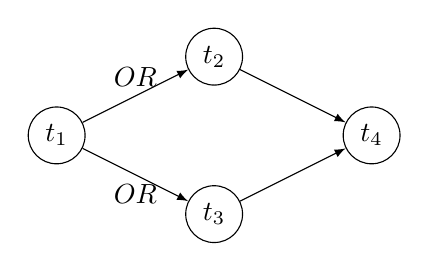
\begin{tikzpicture}
\tikzset{vertex/.style = {shape=circle,draw,minimum size=1.5em}}
\tikzset{edge/.style = {->,> = latex}} 
%\draw (0,0) circle [radius=0.5];
\node[vertex] (a) at  (0,0) {$t_{1}$};
\node[vertex] (b) at  (2,1) {$t_{2}$};
\node[vertex] (c) at (2,-1) {$t_{3}$};
\node[vertex] (d) at (4,0) {$t_{4}$};
\draw[edge] (b) to (d);
\draw[edge] (c) to (d);
\path[-latex]
(a) edge node[above] {$OR$} (b)
(a) edge node[below] {$OR$} (c);
\end{tikzpicture}
\caption{Separation of duty}
\label{fig:Separation of duty}
\end{figure}

\section{Binding of Duty}

\chapter{Implementation}

\chapter{Evaluation}

\chapter{Conclusion}

\chapter{Appendix A: How to Use}

\bibliography{Master}

\end{document}
